\documentclass{article}
\usepackage[utf8]{inputenc}
\usepackage{geometry}
 \geometry{
 a4paper,
 total={175mm,265mm},
 left=15mm,
 top=15mm,
 }
\usepackage{amsmath}
\usepackage{cleveref} %cleverref needs to stand below amsmath package.
\usepackage{graphicx}
\usepackage{float}
\usepackage{url} %To be able to use url in references
\usepackage{graphicx}
\usepackage{tabularx} % in the preamble
\usepackage{wrapfig}
\usepackage{comment}

\usepackage[toc,page]{appendix}

\title{Manual: Productivity lock your phone, lower your dependency on google, and replace Operating System and google calendar synchronisation with an opensource alternative.}
\author{Name: ...}
\date{18-04-2018}
\begin{document}
\maketitle
\tableofcontents
%\setcounter{chapter}{-1} 
 %\setcounter{section}{-1}
\section{Introduction}\label{sec:introduction}
Hi, this contains the manual of how to set up a completely locked phone that does not allow sogging. There are two ways to achieve this if you have the right phone:
\begin{enumerate}
    \item Shortcut: If you already implemented this guide once, and wish to restore your complete system on your phone from a titanium backup file go to: \cref{sec:restore_with_titanium_backup}. 
    \item Implement all the steps described in this manual once, from top to bottom. (after that you can do it the easy way.)
\end{enumerate}
For a complete list of apps that I like to use in this system, see \cref{app:C}.


 \section{Bottlenecks: Current possible phone models for this setup}
There are two bottlenecks to using this guide to apply this productivity lock on your phone:
\begin{enumerate}
    \item Your phone might not be (easily) rootable (yet). Rooting generally requires you to enable some kind of access right, followed by retrievel of a code unique by your phone, which you can submit to your manufacturer, which supplies you with an unlock code, entering that gives you certain rights in your phone. Either at that point it is already rooted, or you need an additonal app that, after those rights have been granted to you, do the actual rooting. Since the procedure varies per phone I did not take the time to document the procedure, you'll have to research this yourself. If you are determined to implement this system but do not know where to start with rooting your phone, feel free to contact me.
    \item Your phone might not be supported by the Open Source operating system lineage for android. You can check this at: \url{https://download.lineageos.org/}
\end{enumerate}
 \section{How to root phone (Exampled Moto G3 Out of 2015)}\label{sec:ch2}
\textbf{This is the manual that I followed, sorry but this is phone dependent so you'll have to look up how to do it or ask a friend.} Todo: make this in a concise short list of instructions.
Source: \url{https://motog5.net/unlock-bootloader-install-twrp-root-moto-g3/}

Pre-Requisites
The device which you are going to root should have a decent amount of battery. We suggest your device is having at least 80\% of battery in it.
Enable USB debugging on your smartphone. Go to Settings > About Phone and tap on build number 8 times. Return to Settings and then go to Developer Options. Enable USB debugging from here.
If you have valuable data, create a backup of all the information which is present in your device. All your data will be erased at the stage you are going to unlock the bootloader of the device.
Install Minimal ADB and Fastboot tools on your PC.
Install drivers of Moto G3 on your PC.
Extra Note: If you enjoyed android apps and games on your Moto G and wanted them on you PC, you can do so just by downloading and installing Bluestacks android emulator. Here are blue stacks system requirements to run blue stacks without error. Check now.

How to unlock bootloader of Moto G 3rd gen
To get root access on Moto G 3rd gen, the bootloader of your device should be unlocked first. Follow the guide shared below as it will help you to unlock the bootloader of Moto G 3rd gen.

Power off your Motorola Moto G smartphone. Once your device is powered off, you need to switch it on in Fastboot mode. To enter the Fastboot mode of Moto G 3rd gen, you have to press Volume Up + Power key.
Connect the smartphone to your PC. Once your device is connected, go to the folder  where you have installed Minimal ADB and Fastboot tools. You need to enter a couple of commands now. Open the command window by selecting right mouse button and Shift key. Select open command window here.
Check if Moto G is connected in Fastboot mode with your PC by entering the command mentioned below.
fastboot devices

Now you need to get the unlock data which will help you to unlock the bootloader of your smartphone. You can enter the command shared below which will assist you in getting unlock key data.
fastboot oem get\_unlock\_data

A long string will be displayed in front you. Copy it and keep it in Notepad. Remove all the spaces which are present in the string.
The next step is opening the Motorola website. Go to the link and open Motorola website.
Create a new Motorola account if you are not having one. Once you are logged on the site, you have to paste the string which you have copied in notepad in Step 5.
Copy it and then select Can my device be unlocked. Select I Agree on the option, and after that, you have to choose Request Unlock Key.
Open your mail id which you used for logging on the Motorola website and then check the mail sent by Motorola. It will have a unlock code which will help you to unlock the bootloader of Moto G3
Open the command window again and enter command mentioned below which will finally unlock the bootloader of Moto G3.
fastboot OEM unlocks (insert code here)

This will unlock the bootloader of Moto G 3rd generation. Now you are ready to install recovery and root your device.

How to install TWRP recovery on Moto G 2015
To install TWRP recovery, you need to download the recovery first.
Download TWRP(2.8.7-r7.img) recovery for Moto G by opening this link. Rename the recovery to img and copy it to the directory of MinimalFastboot and ADB tools.
Now you have to put your device in Fastboot mode again. Repeat Steps 1 and two here which you followed while unlocking the bootloader.
Enter the command mentioned below as it will flash recovery on your device.
fastboot flash recovery twrp.img

Within a couple of minutes, recovery will be flashed on the device.
Once TWRP recovery is flashed, you are ready to root  Moto G3.

Also Read: – All about Motorola Moto G3

How to root Moto G3
Download SuperSU on your mobile by opening this link.
Once downloaded power off your smartphone and enter the recovery by pressing Power + Volume Down button.
Select Install button and browse Super SU file.
Flash the file on your device.
You will get root access on Moto g 3rd gen. This is how you can quickly unlock bootloader and root Moto G 3rd gen.

How to Root Moto G on any Android Firmware
The first thing you have to do is to go to this page.
From the above mentioned site, you have to download the latest version of the Superboot app.
Place the downloaded file on your PC.
Unzip the file anywhere for example on a desktop.
On your computer open a command prompt window (start – run – cmd).
On the command prompt window navigate to the folder you have just unzipped (using cd commands).
Turn off your Moto G smartphone.
Wait a few seconds and then reboot into bootloader mode.
For bootloader mode press and hold volume down and power buttons at the same time for a few seconds.
Then connect your smartphone to your computer via a USB cable.
On the cmd window type the following command: “superboot-windows.bat.”
Wait while your Moto G is being rooted.
In the end, unplug the USB cord and reboot your phone.
Go to Google Play and download the Root Checker app to check the root status.
If root checker app says, root access available then Enjoy you have rooted your Moto G.
After Moto G rooting, you can install custom ROM’s and firmware.
Note: – If you want to remove the unlocked bootloader message then just download this file and flash it via TWRP recovery.


 \section{Installing a different BOOT/Phone Bios software. E.g.: TWRP}\label{sec:ch3}
Still need to document how ti install TWRP, I think you download a zip from somewhere that contains the bios, then store it somewhere on your internal storage of your phone, after you have rooted your phone, and then restart your phone in recovery mode.
%TODO: Document how to install TWRP on your phone
\subsection{Booting in TWRP after installation of TWRP}\label{sec:t2_back}
To boot into TWRP:
\begin{enumerate}
    \item shut down phone
    \item in moto 3rd g: press power+volume down button to start up.
    \item select recovery mode
    \item press powerbutton to chose recovery mode
\end{enumerate}

 \section{Install different phone OS. E.g.: linneageOS}\label{sec:ch4}
\begin{enumerate}
    \item download addonsu-14.1-arm-signed.zip
    \item and download lineage-14.1-20181120-nightly-osprey-signed from: https://download.lineageos.org/osprey (for moto g3 take moto g 2015)
    \item download adb minimal (use it by opening the file py\_cmd.exe)
    \item copy addonsu-14.1-arm-signed.zip as "lineage.zip" into folder "Minimal ADB and Fastboot\_techbeasts".
    \item boot in twrp
    \item copy the .zip to the phone when booted in twrp with command:
\begin{verbatim}
adb push <source-path> <target-path>    
\end{verbatim}

    \item in twrp install addonsu-14.1-arm-signed.zip.
\end{enumerate}

 \section{Get root access. E.g.: SuperSU}\label{sec:ch5}
 \section{Remove recent apps button from navigation bar. E.g.:  App custom navigation bar}\label{sec:ch6}
\subsection{Introduction}
This assumes you just did a fresh install of LineageOS osprey 14.1 nightly build.
\subsection{Steps:}
\begin{enumerate}
    \item download fdroid
    \item download terminal emulator from fdroid
    \item download custom navigation bar from an alternative source such as: \url{https://www.apkmirror.com/apk/paphonb/custom-navigation-bar/custom-navigation-bar-0-8-11b-release/custom-navigation-bar-0-8-11b-android-apk-download/download/}
    \item rename it to customNavBar.apk, install it. (it was named: \url{xyz.paphonb.systemuituner_0.8.11b-118_minAPI24(nodpi)_apkmirror.com.apk} with command:
\begin{verbatim}
adb install customNavBar.apk
\end{verbatim}
    \item Then give custom navigation bar root access from adb with command:
\begin{verbatim}
adb shell pm grant xyz.paphonb.systemuituner android.permission.WRITE_SECURE_SETTINGS    
\end{verbatim}
    \item once that is done, ignore the next command you are supposed to enter in the android terminal emulator listed below. (I entered it several times but it kept saying I should grant runtime access. That is done with the adb command above. After the adb command above I did not re-enter the command below. (But just in case it did influence the procedure here it is):
\begin{verbatim}
pm grant xyz.paphonb.systemuituner android.permission.WRITE_SECURE_SETTINGS    
\end{verbatim}
    \item Then open the custom Navigation bar app.
    \item do the compatibility test. It should change the home button to the little arrow shown in the middle of \cref{fig:diag}.
    
    \begin{figure}[H]
        \centering
        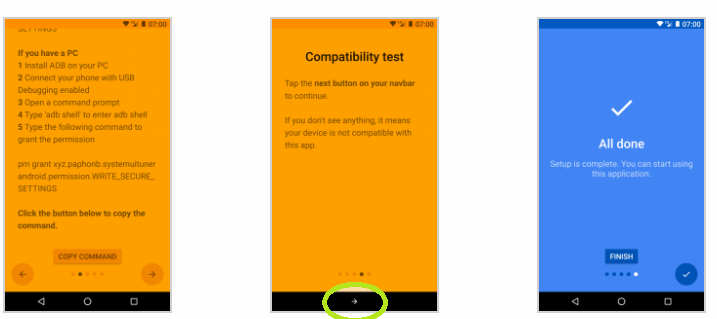
\includegraphics{images/pic.png}
        \caption{If the custom navigation app works with your phone the diagnostic test should change the home button as shown in the green circle.}
        \label{fig:diag}
    \end{figure}
    \item Next, in the app click "experimental features" and remap the "overview " button to "home".
    \item that's it. Now quickly reboot and uninstall the app as it shared your data. (The remapping will remain active after de-installation!
\end{enumerate}
 \section{Install lot of apks at once. E.g. adb minimal}\label{sec:ch7}
Use the command:
\begin{verbatim}
for %f in (C:\your_app_path\*.apk) do adb install "%f"    
\end{verbatim}

 \section{Automatic periodic data backups. E.g.: app tasker}\label{sec:ch8}
To create the task that automatically exports the specific data listed in \cref{subsec:mob_to_pc}, do the following:

This is like a double safety data backup and data overview for convenience.

\begin{enumerate}
    \item open tasker
    \item then in the top bar where it says "profiles.. tasks .." hold "tasks>import" then select the file named "CopyWhatsappV0.prj.xml" import that task.
    \item You can create that file by opening a notepad and pasting the content of \cref{app:A} in it and then renaming the .txt file to a .xml file.
    \item that copies all your whatsap data into a folder on the external storage (drive named 17EE-2356) named: WhatsAppExport
    \item Todo: verify this method works.
\end{enumerate}


\subsection{Export automatic periodic backups with Tasker}
Using tasker you can export the data manually from internal SD to External SD. To export your whatsapp media, import the tasker project=(task executed every xx [time span] listed in \cref{app:A}. \cref{app:A} contains the the xml code for the .xml file that is a tasker project (copy the text into a notepad and store it as WhatsappExport.xml). If you import this project it will automaticallly export your files every night to external SD. In \cref{app:F} a different tasker project is listed that exports all non-Whatsapp media to your external SD. %TODO: list exact files and folders, and folder types
%TODO: Make it dynamic, so that it asks the user to select the folder locations once.
\subsubsection{Download files from phone to laptop through USB}\label{subsec:mob_to_pc}
\begin{enumerate}
    \item Open 
\begin{verbatim}
../Minimal ADB and Fastboot_techbeasts/py_cmd.exe    
\end{verbatim}

    \item Connect Phone through USB with PC. (Verify it is connected G, by typing
\begin{verbatim}
"adb devices" in py_cmd.exe (should return a code for the device))    
\end{verbatim}
    \item Enter the following commands to copy their respective folder:
\begin{verbatim}
adb pull "/storage/17EE-2356/WhatsAppExport" "E:\2018-09-22 backups\Android\WhatsAppExport" 

adb pull "/storage/17EE-2356/DCIM" "E:\2018-09-22 backups\Android\DCIM"

adb pull "/storage/17EE-2356/call records" "E:\2018-09-22 backups\Android\call records" 

adb pull "/storage/17EE-2356/Contacts" "E:\2018-09-22 backups\Android\Contacts"

adb pull "/storage/17EE-2356/titanium backups" "E:\2018-09-22 backups\Android\titanium backups"    
\end{verbatim}
\end{enumerate}
\subsection{List of data that is exported: (this data is only put there if you have automated the tasker backup as described in \cref{sec:tasker_auto_backup}}
\begin{enumerate} 
    \item WhatsAppExport
    \item DCIM
    \item call records
    \item Contacts
    \item Titanium backups
\end{enumerate}
\subsubsection{Create a batchscript to do the absorbing.}
Specifications:
\begin{enumerate}
    \item get list of folders on phone.
    \item get single destination folder
    \item automatically create subdestinations in destination folder based on list of folders on phone, if the destinations do not already exist.
    \item for all files in folder pull. (duplicate files are just overwritten)
    \item \textbf{Todo:} for all files: if file is created a week ago, and file is on pc in destination folder, then delete on phone.
    \item \textbf{Todo:} Structure backup location and make it dynamic.
\end{enumerate}


 \section{Setup automatic app and settings backup. E.g. titanium backup pro}\label{sec:tasker_auto_backup}
There are two options, either download version titanium backup 7.4 +patch, or dld titanium backup 8.0 from Mega:  \url{Mega.co.nz}. Then instal titanium backup.

\begin{enumerate}
    \item First install supersu: by copying addonsu-14.1-arm-signed.zip to the phone with for example:
\begin{verbatim}
adb push <source-path> <target-path>    
\end{verbatim}
 
    \item Next download titanium 8.0. 
    \item then install it. It will say will not work has no root permission.
    \item So go to settings and enable developer options by tapping the android type 7 times. 
    \item go into settings, developer options and enable root access (for apps and adb).
    \item restart
    \item open Titanium backup and it works.
    

\end{enumerate}

\section{Restore old backup with Titanium Backup}\label{sec:restore_with_titanium_backup}
Import a  ... file and hit "restore".
\subsection{Limitations: Titanium backup w.r.t. Whatsapp}
You can not merge different backups of whatsapp yet, so suppose you have a really old backup of whatsapp and you hope whattsapp automaticallyy downloads the missing messenges your number received between "now and the time of the backup", you're in tough luck. So the solution/best approach is to just maintain a consistent backup procedure and restore the latest backup as quickly as possible after a reset. That way the WA message gap is minimalised. 



 \section{Enable remote keyboard}\label{sec:remote_keyboard}
\begin{enumerate}
    \item 0.First open remote keyboard.
\item 1.(Go to phone settings and enable remote keyboard as keyboard)
\item 2.Then go to app remote keyboard and also there, enable remote keyboard as keyboard.
\item 3.Then on pc>control panel ctrl+F "turn windows features" on or of 
\item 4.Enable Telnet Client my marking the checkbox as shown in \cref{fig:remote_keyboard}.
\begin{figure}[H]
    \centering
    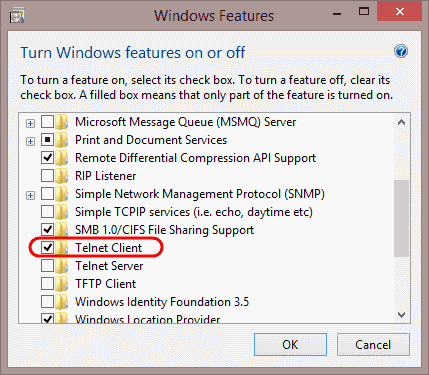
\includegraphics{images/remoteKeyboard.png}
    \caption{How to enable telnet on Windows 10}
    \label{fig:remote_keyboard}
\end{figure}
\item 5. Then start cmd and enter:
\begin{verbatim}
 telnet <ip from remote keyboard app> <port>
(including the space)
\end{verbatim}
\item 7. Then from attached calendars.ods 
    \begin{enumerate}
        \item 7.1 (When you manually add a calender by copying the google id as described here Make            sure the space after the calender id/email is gone!! so that the "/events" is also                        included.)
        \item 7.2 Use that to quickly copy calendars.ods column D into DAVdroid, (Copy column D, then paste it in the phone by rmb on cmd screen)
    \end{enumerate}
    \item 8. Open davdroid
\end{enumerate}





\section{Auto Sync all google calendars through davdroid}\label{sec:ch10}
\begin{enumerate}
    \item In public github download the PublicCodeLibrary/VBA/Google Davdroid calendar app sync/ folder. Or in excel/Google Davdroid Calendar App Sync/.
    \item Open the Excel named "calendars from gmail to davdroid V14.xlsm". That downloads google calendar website, and controls your phone.
    \item open \url{https://calendar.google.com/calendar/r/week?pli=1}
    \item Save that website as: "google.txt" in the subfolder "WebsiteSource" which is located in the same folder as the excel.
    \item install remote keyboard on phone as explained in \cref{sec:remote_keyboard} and make sure you can control phone from cmd with command: 
\begin{verbatim}
 telnet <ip from remote keyboard app> <port>
(including the space)
\end{verbatim}
    \item For me:

    \item Download opensource ahk from: \url{https://www.autohotkey.com/download/}
    \item Put the cmd with the remote keyboard connection in the right half of your screen.
    \item put the excel in the left hand side of your screen.
    \item Open davdroid on your phone, (such that the plus symbol is clickable, though do not click it.)
    \item Press the "0. get cal codes" 
    \item press the cmd with remote keyboard logged in in it, then immediately afterwards press "1. Copy Data to Phone".
\end{enumerate}

\subsection{Deleting all calendars out of Davdroid at once:}
There are at least two ways to do this:
\begin{enumerate}
    \item \textbf{Do every time:} Run the APK resetDavdroid.
    \item Do once: (Download, install and ) run app: "resetDavdroid".
    \begin{enumerate}
        \item On your external SD card create a folder named: "DAVdroidInstal" and copy the davdroid installation APK. You can get it by going to: \url{https://f-droid.org/en/packages/at.bitfire.davdroid/} and clicking: "Download APK". (currently that leads to: \url{https://f-droid.org/repo/at.bitfire.davdroid_254.apk}.
        \item rename the downloaded apk installation file to: at.bitfire.davdroid.apk
        \item Determine the location of your SD-card in your phone, in my phone it was /storage/17EE-2356. substitute the location of your SD card into the .xml code in \cref{subsubsec:taskResetDavdroid}:
        \item Copy Then copy the text of \cref{subsubsec:taskResetDavdroid} into a notepad file called resetDavdroid.txt and rename the file into resetDavdroid.xml.
        \item Import the .xml in tasker.
        \item Pick an icon for the task
        \item Export the task to an apk and install the apk:
        \begin{itemize}
            \item long press the task then three dots in top right 
            \item Package: name it to for example a.b.com
            \item Advanced Configuration: Check the box
            \item At Extra permissions enter:
\begin{verbatim}
android.permission.WRITE_SECURE_SETTINGS
\end{verbatim}
            \item That exports the app to: (Internal) storage card/media/tasker/factory/kids/ 
 .apk which in my case had the exact path name:
\begin{verbatim}
/storage/emulated/0/Tasker/factory/kids/
\end{verbatim}       
        \end{itemize}
        \item ..Then run the app to reset Davdroid. That clears out all calendars. 
            \begin{enumerate}
                \item When it prompts for root access, mark "do not ask again" and press OK.
                \item When then applock asks to lock (the freshly installed) Davdroid click Cancel/NO.
                \item (Actually export/build and install- the app by pressing the back button on the top left of the screen).
            \end{enumerate}
    \end{enumerate}
\end{enumerate}
\subsubsection{.xml code reset Davdroid task}\label{subsubsec:taskResetDavdroid}
\begin{verbatim}
<TaskerData sr="" dvi="1" tv="5.2.bf1">
    <Task sr="task28">
        <cdate>1546182301418</cdate>
        <edate>1546204083437</edate>
        <id>28</id>
        <nme>ResetDAVdroid</nme>
        <pri>100</pri>
        <Kid sr="Kid">
            <eperm0>android.permission. WRITE_SECURE_SETTINGS</eperm0>
            <launchID>28</launchID>
            <pkg>a.b.com</pkg>
            <vnme>1.0</vnme>
            <vnum>4</vnum>
        </Kid>
        <Action sr="act0" ve="7">
            <code>123</code>
            <Str sr="arg0" ve="3">pm uninstall at.bitfire.davdroid</Str>
            <Int sr="arg1" val="0"/>
            <Int sr="arg2" val="1"/>
            <Str sr="arg3" ve="3"/>
            <Str sr="arg4" ve="3"/>
            <Str sr="arg5" ve="3"/>
        </Action>
        <Action sr="act1" ve="7">
            <code>123</code>
            <Str sr="arg0" ve="3">pm install /storage/17EE-2356/DAVdroidInstal/at.bitfire.davdroid.apk</Str>
            <Int sr="arg1" val="0"/>
            <Int sr="arg2" val="1"/>
            <Str sr="arg3" ve="3"/>
            <Str sr="arg4" ve="3"/>
            <Str sr="arg5" ve="3"/>
        </Action>
        <Img sr="icn" ve="2">
            <nme>hd_content_discard</nme>
        </Img>
    </Task>
</TaskerData>
\end{verbatim}
For me the location is: %mega8/mob/18-12-30 custom Apps/

\subsection{TODO:}
\begin{enumerate}
    \item Get calendars through api
    \item correct long names of imported .cal files from mytimetable
    \item automate adapting loop of .ahk to nr of calendars.
    \item stop doing beun de haas and just do it all inside the smartphone.
    \item check if opentasks has a better calendar synchronization than taskwarrior andorid task apk.
\end{enumerate}
\subsection{Try to write the calendars directly into the phone storage for Davdroid}
Davdroid does not store any calendars, those are stored in their normal place in the android operating system. However, it uses a file services.db to change those files is what I understood. The changing happens using sql. The following things are unclear:
\begin{itemize}
    \item It is unclear wether the davdroid settings are stored in the services.db or whether the services.db is just a sort of api/handler that accesses the calendar settings of davdroid somehow.
    \item Are there a lot of extra settings changed within Davdroid when you add a calendar the conventtional way. E.g. If I happen to find the location where the calendar settings of Davdroid are stored, and I would be able to perfectly replicate add a calendar there (by for example, first adding one just using davdroid correctly, copying the file content that contains that specific calendar setting, and deleting and re-installing davdroid (including data) and restoring that specific calendar file content in that calendar-settings-file.) Or are there separate processeses like for example encryption keys uniquely created if you verify for example the base url in the normal davdroid way, which I did not do by simply pasting in the calendar settings?
    \item Where are the actual settings stored, derive that from the answers given by rc2822.
    \item How to decrypt/encrypt/store the passwords for the gmail acocunt?
\end{itemize}
 So presumably, you want to find the services.db to see how you can inject your calendar settings into davdroid.
Source: \url{https://forums.bitfire.at/topic/1834/location-of-calendar-settings-storage-on-lineageos-14-1-with-davdroid-1-11-4-1-ose/6}
Services.db is not found, however, a similar calendars.db is found at location:
\begin{verbatim}
/data/data/com.android.providers.calendar/databases/calendar.db
\end{verbatim}
This contains at least the list of calendars of android itself, it is not yet sure if it also contrains the synchronisation settings of davdroid.



\begin{enumerate}
    \item The services.db is located in the root as: /data/data/at.bitfire.davdroid/databases/services.db
    \item To read the services.db file look at: \url{https://developer.android.com/studio/command-line/adb#othershellcommands}
    \item with adb and the following commands you can manipulate the database file:
\begin{verbatim}
adb -s emulator-5554 shell
sqlite3 /data/data/com.example.app/databases/rssitems.db
SQLite version 3.3.12
Enter ".help" for instructions
\end{verbatim}    
\item 

https://www.sqlite.org/download.html

\item Found the services.db file relative to the root of my devices as: /data/data/at.bitfire.davdroid/databases/services.db
\item Exported and visually inspect the database with SQlite studio to determine which tables the services.db contain.
\item That allows for conversion of the services.db to a .csv file according to: \url{http://www.sqlitetutorial.net/sqlite-tutorial/sqlite-export-csv/.}
\item That allows for reverse engineering the database, to generate new ones with custom calendars.
\item The next step however, is to determine where and how the password is stored by Davdroid, for for example the accompanying google accounts for base-url added google calendars.
\item the password is stored (in plain text in 2016) in androids default location using the android account manager: \url{https://developer.android.com/reference/android/accounts/AccountManager#setPassword%28android.accounts.Account,%20java.lang.String%29} and \url{https://developer.android.com/reference/android/accounts/AccountManager#getPassword(android.accounts.Account)}. That could mean you should use an api to get the password. 
\item According to \url{https://forums.bitfire.at/topic/264/view-changes-properties-of-an-existing-davdroid-account/21} the passwords are stored in /data/system/users/0/accounts.db. I have not yet been able to find that database but I will look into it in more detail.
\end{enumerate}
\noindent Using 
 \section{Setup Applock}\label{sec:ch11}


ADB Applock (Note. FIRST DO TITATNIUM BACKUP, you will not be able to modify titanium backup after setting up the lock!" 

\noindent Also, First set up the lock with a code you know so you can practice. TEST IT FOR A WEEK! Then if everything is perfect (you can access what you need when you need it without the unlock code) let a friend change the code. (And or, if you're hardcore, let him/her hide the applock application from the appview (inside applock)).


\noindent Open applock press the half moon on the bottom left to see the locking profiles. Then add the following, and any apps that you also use to procrastinate to the list. An example list is found in \cref{app:b}.

\newpage
Create new profile named "Lock day" and Lock (save when done locking):


\section{Retrieving data from a (TWRP) brick with ADB:}\label{sec:ch12}
%\setcounter{subsection}{-1}
\subsection{Scenario:}
You tried to change the navigation bar, but now your phone will boot but the screen is black and phone is responsive but you cant do anything except reboot, power down and ...

Luckily you can still connect with adb devices to the phone, as "adb devices" returns your device(code)
\subsection{backing up the sdcard:}
\begin{enumerate}
    \item download adb devices
    \item get the location of the sdcard with:
\begin{verbatim}
adb shell echo $EXTERNAL_STORAGE
\end{verbatim}
    \item get the location of the "internal sd card with command (sounds nice but does not work): 
\begin{verbatim}
adb shell echo $INTERNAL_STORAGE    
\end{verbatim}
    \item Copy all content of the sdcard to your pc with command:
\begin{verbatim}
adb pull "/sdcard/" "E:\\2018-11-20_android_sdcard_backup\\"    
\end{verbatim}    
\item to copy the other storage location (sdcard appears to be the internal storage):
\item 
\begin{verbatim}
adb pull "/mnt/sdcard/" "E:\\2018-11-20_android_sdcard_backup\\"
\end{verbatim}   
\item and:
\begin{verbatim}
adb pull "/storage/17EE-2356" "E:\\2018-11-20_android_sdcard_backup\\"    
\end{verbatim}
\begin{verbatim}
adb pull "/storage/emulated" "E:\\2018-11-20_android_sdcard_backup\\"
\end{verbatim}
\begin{verbatim}
adb pull "/storage/self" "E:\\2018-11-20_android_sdcard_backup\\"
\end{verbatim}
\end{enumerate}

\subsection{Gained knowledge}
\begin{enumerate}
    \item You can open a sort of Linux terminal in your phone with the command:
\begin{verbatim}
adb shell
\end{verbatim}
    \item then command "ls" lists the directories in that folder. You can change directories with cd.
    \item Then if you completely browse up the hierarchie with "cd .." you can see where the external olders are located if you dive back into the directories smartly.
    \item that yielded a location of: 
\begin{verbatim}
/storage/17EE-2356
/storage/emulated
/storage/self
\end{verbatim}
    
\end{enumerate}
\section{Connecting to WIFI}
To be able to connect to a wifi you're going to add a wifi connection manually in the phone. 

\subsection{Do Once: download and install}\label{subsec:wifi_once}
\begin{enumerate}
    \item "wifi analyzer" \url{http://apkfind.com/dl5/apk/2018/4/8/com.farproc.wifi.analyzer_139.apk?id=com.farproc.wifi.analyzer&f=Wifi%20Analyzer_3.11.2_apk-dl.com.apk}. 
    
    \item "Wifi connecter Library" \url{http://apkfind.com/dl5/apk/2016/11/8/com.farproc.wifi.connecter_16.apk?id=com.farproc.wifi.connecter&f=Wifi%20Connecter%20Library_2.0.3_apk-dl.com.apk}
    \item Install QuickEdit from \url{https://apk-dl.com/quickedit-text-editor-writer-code-editor/com.rhmsoft.edit}
    \item Install the "Edit wifi settings" "app" I created, OR:
    \item you can create it yourself with tasker by importing the task xml code listed in \cref{app:E} and exporting the task as APK. (this way you can open the wifi settings after tasker and your file explorer have been locked by the productivity lock).
    \begin{enumerate}
        \item For Tasker V5.2.bf1 You are required to get the exact same tasker factory version as you have the Tasker app version. The steps required to create the task and consequently the app, were: 
        \item Create a new task in Tasker. 
        \item Press the "+" symbol. 
        \item Click "Code". 
        \item Select "Run Shell" 
        \item At command, enter:
\begin{verbatim}
am start -a android.intent.action.VIEW -c android.intent.category.DEFAULT -d "file:///data/misc/wifi/wpa_supplicant.conf" -t "text/plain"    
\end{verbatim}        
        \item Leave Timeout(Seconds) at 0 
        \item Mark the checkbox at: "Use Root" 
        \item Leave the rest blank/unchanged. 
        \item Hit the back arrow. 
        \item Now you can run the task by pressing the "play" button in the bottom left.
        \item To export the task as an app first install taskbuilder from \url{https://apkpure.com/tasker-app-factory/net.dinglisch.android.appfactory/download?from=details}
        \item Select an icon for the task (9 bloks bottom middle of screen.)
        \item Long press task>export>as app.
        \item The file was only openable by the QuickEdit app. The others did not get access.
    \end{enumerate}
    \begin{figure}[H]
        \centering
        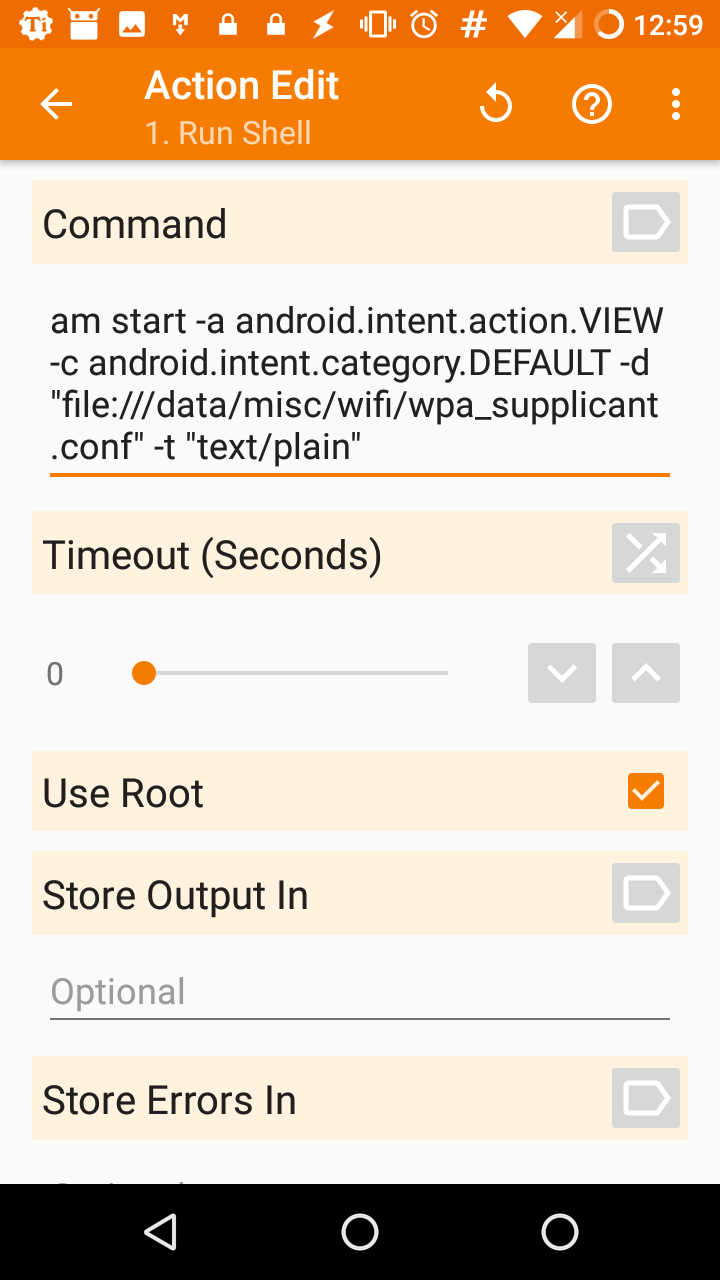
\includegraphics[width=10cm,height=10cm,keepaspectratio]{images/tasker.png}
        \caption{Example of the input in the task at tasker}
        \label{fig:my_label}
    \end{figure}
    
\end{enumerate}

\subsection{Do everytime you connect to a NEW, UNKOWN wifi network}
\begin{enumerate}
    \item Find the BSSID using the app "wifi analyzer" and copy it.
    \item Open the "OpenWifiSettings" app (from cloud, or created with Tasker or restored from Titanium backup) (this opens the wifi configuration file in app "QuickEdit".
    \item Now you want to create the network settings directly in the file where android normally stores it if you add a new wifi network through network settings. To make it easier you can:
    \item OPTION I: Use the template given in \cref{app:D}, by copying an example network of that text. 
    \item OPTION II: OR you can let the app "full wifi" create a new template for that network for you. Either way you still need to know what the netwerk settings must be. In "full wifi:" \textgreater Click: add new network\textgreater select required settings\textgreater 
    \item Next, open the app "OpenWifiSettings".
            \begin{itemize}
            \item OPTION I: If it exists remove the network settings for that BSSID. Then add the text of the network you copied from \cref{app:D} and modify the settings/text (e.g. BSSID, password, username, authentication method etc) to what they need to be for your new network.)
            \item OPTION II: Find the BSSID and edit the settings to what they should be, if you  
            \item Save the file by long pressing the pencil symbol in the top right of QuickEdit.
        \end{itemize}

    \item Turn wifi on and of to re-initialize the modified //data/misc/wifi/wpa\_supplicant.conf file.
    \item After storing the connection settings for a specific wifi network, you can connect to it in (at least) 2 ways:
    \begin{itemize}
        \item You can connect by clicking the wifi network name(ssid) in the dragdown screen/widget from the normal android homescreen. But that might bring you to wifi settings (which are locked with applock) and ask for a password the first time, click backbackback till you're in the homescreen again without entering any pathword. It will now connect to the ssid you've chosen, or else retry. 
        \item Or you can open the app "wifi analyzer" and long press the wifi network ssid, press connect. It should then automatically connect to the wifi. If you cannot press connect without entering a password, you did not enter the correct data in the wpa\_supplicant.conf file. Please retry.
        
    \end{itemize}
    \item Todo: Create a tasker apk replaces the normal wifi settings interface of android. By asking the user for the input using a dropdownbox listing connection type options and password etc, to prevent typos in the .conf file. 
\end{enumerate}

\section{Summary Tasker}
Tasker is used for the following applications. (how it is used in tasker){what the filetype is stored as}:
\begin{enumerate}
    \item Copying the whatsapp media (as task and profile at 3:42-5:00) {Cloud:xml,.prf.xml}
    \item Copying the camera images (as task and profile at 3:00-3:40){Cloud:xml,.prf.xml}
    \item App to open wifisettings (task named OpenWifiSettings3){Cloud:xml,apk}
    \item app to reset Davdroid (task named ResetDAVdroid){Cloud:xml,apk}
    \item app to reset Taskwarrior (task named ResetTaskwarrior){Cloud:xml,apk}
\end{enumerate}

\section{Downloading data from phone:}
Open location of sdcard with: 
\begin{verbatim}
adb shell cd $EXTERNAL_STORAGE    
\end{verbatim}
List files in Sdcard with:
\begin{verbatim}
adb shell ls $EXTERNAL_STORAGE    
\end{verbatim}
Copy file from External SD card:
\begin{enumerate}
    \item adb root
    \item adb shell cd root
    \item adb shell df
    \item Inspect those values to get the path of the external sd card. For me it was:
\begin{verbatim}
/mnt/media_rw/17EE-2356
\end{verbatim}
    \item copy the file to the location of your "py\_cmd.exe" with:
\begin{verbatim}
adb pull /mnt/media_rw/17EE-2356/contacts.vcf
\end{verbatim}
\end{enumerate}

\section{Softbricked your phone again with incorrect wifi edit}
\subsection{Scenario}
If you copy paste a wifi from the text editor and don't add the correct code at the bottom, you softbrick your phone. To fix it:

\subsection{If you need immediate reboot, losing wifi settings}
\begin{enumerate}
    \item hold power+volume down.
     \item recovery mode
    \item advanced
    \item file manager,
    \item browse to
    \item \verb+/data/misc/wifi/wpa_supplicant.conf+
    \item rename the file to
    \item \verb+adb pull /data/misc/wifi/wpo_supplicant.conf+
    
    \item now you can reboot safely but lost your wifi. To fix your wifi settings again (by removing the invalid one).
\end{enumerate}


\subsection{Unbrick and keep wifi settings}
\begin{enumerate}
    \item open \verb+py_cmd.exe+ in for example \verb+c:/path with space/py_cmd.exe+
    \item adb devices
    \item (wpa if you did not change the name)
    \item \verb+adb pull /data/misc/wifi/wpo_supplicant.conf+
    \item Delete messed up entry from conf file with notepad.
    \item rename file to \verb+wpa_supplicant.conf+
    \item \verb+adb push "c:/path with space/wpa_supplicant.conf" /data/misc/wifi/wpa_supplicant.conf+

    \item for me: 
\begin{comment}
adb root

adb push "E:/18-09-19 Document structure/personal/Automation and Systems/Android/2018-09-22 transfer and adb/Minimal ADB and Fastboot_techbeasts/wpa_supplicant.conf" ///data/misc/wifi/wpa_supplicant.conf
\end{comment}
\end{enumerate}

\subsection{lesson}
To add a new wifi network:
\begin{enumerate}
    \item open the app wifi analyzer, 
    \item and press the wifi network you want to add, 
    \item then enter a password
    \item store the network
    \item Then open self "created" (tasker) app open wifi settings and change the password.
    \item \textbf{DO NOT COPY PASTE AN EXISTING WIFI NETWORK TO MODIFY IT,THAT WILL SOFTBRICK YOUR PHONE}
\end{enumerate}

\input{Chapters/conclusion.tex} \newpage

\begin{appendices}
%\chapter{Tasker copy to external sd xml file}
\end{appendices}
\appendix
\section{.xml files for Tasker V5.2.bf1 Whatsapp media Profile}\label{app:A}
\subsection{Whatsapp automatic backup of all media (except messages)}
A project in tasker V5.2.bf1 is, (in this case) a time schedule, (every day at 01:37 in the night), that executes a list of tasks. To import this project into tasker V5.2.bf1, Save code below as a .xml file and then longpress "projects" in top bar>import and select this file. (or just install the app (from the titanium backup)). 
\\
\\

\begin{verbatim}
<TaskerData sr="" dvi="1" tv="5.2.bf1">
    <Task sr="task6">
        <cdate>1537598778795</cdate>
        <edate>1543785505373</edate>
        <id>6</id>
        <nme>CopyWhatsappV0</nme>
        <pri>100</pri>
        <Kid sr="Kid">
            <launchID>3</launchID>
            <pkg>roj.iow.mwg</pkg>
            <vnme>v1</vnme>
        </Kid>
        <Action sr="act0" ve="7">
            <code>405</code>
            <Str sr="arg0" ve="3">WhatsApp/Media/WhatsApp Images/</Str>
            <Str sr="arg1" ve="3">/storage/17EE-2356/WhatsAppExport/WhatsApp Images/</Str>
            <Int sr="arg2" val="0"/>
        </Action>
        <Action sr="act1" ve="7">
            <code>408</code>
            <Str sr="arg0" ve="3">WhatsApp/Media/WhatsApp Images</Str>
            <Int sr="arg1" val="1"/>
            <Int sr="arg2" val="0"/>
        </Action>
        <Action sr="act10" ve="7">
            <code>408</code>
            <Str sr="arg0" ve="3">WhatsApp/Media/WhatsApp Animated Gifs</Str>
            <Int sr="arg1" val="1"/>
            <Int sr="arg2" val="0"/>
        </Action>
        <Action sr="act11" ve="7">
            <code>409</code>
            <Str sr="arg0" ve="3">WhatsApp/Media/WhatsApp Animated Gifs</Str>
            <Int sr="arg1" val="0"/>
            <Int sr="arg2" val="0"/>
        </Action>
        <Action sr="act12" ve="7">
            <code>405</code>
            <Str sr="arg0" ve="3">WhatsApp/Media/WhatsApp Voice Notes/</Str>
            <Str sr="arg1" ve="3">/storage/17EE-2356/WhatsAppExport/WhatsApp Voice Notes</Str>
            <Int sr="arg2" val="0"/>
        </Action>
        <Action sr="act13" ve="7">
            <code>408</code>
            <Str sr="arg0" ve="3">WhatsApp/Media/WhatsApp Voice Notes</Str>
            <Int sr="arg1" val="1"/>
            <Int sr="arg2" val="0"/>
        </Action>
        <Action sr="act14" ve="7">
            <code>409</code>
            <Str sr="arg0" ve="3">WhatsApp/Media/WhatsApp Voice Notes</Str>
            <Int sr="arg1" val="0"/>
            <Int sr="arg2" val="0"/>
        </Action>
        <Action sr="act15" ve="7">
            <code>405</code>
            <Str sr="arg0" ve="3">WhatsApp/Media/WhatsApp Stickers/</Str>
            <Str sr="arg1" ve="3">/storage/17EE-2356/WhatsAppExport/WhatsApp Stickers</Str>
            <Int sr="arg2" val="0"/>
        </Action>
        <Action sr="act16" ve="7">
            <code>408</code>
            <Str sr="arg0" ve="3">WhatsApp/Media/WhatsApp Stickers</Str>
            <Int sr="arg1" val="1"/>
            <Int sr="arg2" val="0"/>
        </Action>
        <Action sr="act17" ve="7">
            <code>409</code>
            <Str sr="arg0" ve="3">WhatsApp/Media/WhatsApp Stickers</Str>
            <Int sr="arg1" val="0"/>
            <Int sr="arg2" val="0"/>
        </Action>
        <Action sr="act18" ve="7">
            <code>405</code>
            <Str sr="arg0" ve="3">WhatsApp/Media/WhatsApp Profile Photos/</Str>
            <Str sr="arg1" ve="3">/storage/17EE-2356/WhatsAppExport/WhatsApp Profile Photos</Str>
            <Int sr="arg2" val="0"/>
        </Action>
        <Action sr="act19" ve="7">
            <code>408</code>
            <Str sr="arg0" ve="3">WhatsApp/Media/WhatsApp Profile Photos</Str>
            <Int sr="arg1" val="1"/>
            <Int sr="arg2" val="0"/>
        </Action>
        <Action sr="act2" ve="7">
            <code>409</code>
            <Str sr="arg0" ve="3">WhatsApp/Media/WhatsApp Images</Str>
            <Int sr="arg1" val="0"/>
            <Int sr="arg2" val="0"/>
        </Action>
        <Action sr="act20" ve="7">
            <code>409</code>
            <Str sr="arg0" ve="3">WhatsApp/Media/WhatsApp Profile Photos</Str>
            <Int sr="arg1" val="0"/>
            <Int sr="arg2" val="0"/>
        </Action>
        <Action sr="act21" ve="7">
            <code>405</code>
<Str sr="arg0" ve="3">WhatsApp/Media/WhatsApp Audio/</Str>
            <Str sr="arg1" ve="3">/storage/17EE-2356/WhatsAppExport/WhatsApp Audio</Str>
            <Int sr="arg2" val="0"/>
        </Action>
        <Action sr="act22" ve="7">
            <code>408</code>
            <Str sr="arg0" ve="3">WhatsApp/Media/WhatsApp Audio</Str>
            <Int sr="arg1" val="1"/>
            <Int sr="arg2" val="0"/>
        </Action>
        <Action sr="act23" ve="7">
            <code>409</code>
            <Str sr="arg0" ve="3">WhatsApp/Media/WhatsApp Audio</Str>
            <Int sr="arg1" val="0"/>
            <Int sr="arg2" val="0"/>
        </Action>
        <Action sr="act3" ve="7">
            <code>405</code>
            <Str sr="arg0" ve="3">WhatsApp/Media/WhatsApp Video/</Str>
            <Str sr="arg1" ve="3">/storage/17EE-2356/WhatsAppExport/Whatsapp Video/</Str>
            <Int sr="arg2" val="0"/>
        </Action>
        <Action sr="act4" ve="7">
            <code>408</code>
            <Str sr="arg0" ve="3">WhatsApp/Media/WhatsApp Video</Str>
            <Int sr="arg1" val="1"/>
            <Int sr="arg2" val="0"/>
        </Action>
        <Action sr="act5" ve="7">
            <code>409</code>
            <Str sr="arg0" ve="3">WhatsApp/Media/WhatsApp Video</Str>
            <Int sr="arg1" val="0"/>
            <Int sr="arg2" val="0"/>
        </Action>
        <Action sr="act6" ve="7">
            <code>405</code>
            <Str sr="arg0" ve="3">WhatsApp/Media/WhatsApp Documents/</Str>
            <Str sr="arg1" ve="3">/storage/17EE-2356/WhatsAppExport/WhatsApp Documents/</Str>
            <Int sr="arg2" val="0"/>
        </Action>
        <Action sr="act7" ve="7">
            <code>408</code>
            <Str sr="arg0" ve="3">WhatsApp/Media/WhatsApp Documents</Str>
            <Int sr="arg1" val="1"/>
            <Int sr="arg2" val="0"/>
        </Action>
        <Action sr="act8" ve="7">
            <code>409</code>
            <Str sr="arg0" ve="3">WhatsApp/Media/WhatsApp Documents</Str>
            <Int sr="arg1" val="0"/>
            <Int sr="arg2" val="0"/>
        </Action>
        <Action sr="act9" ve="7">
            <code>405</code>
            <Str sr="arg0" ve="3">WhatsApp/Media/WhatsApp Animated Gifs/</Str>
            <Str sr="arg1" ve="3">/storage/17EE-2356/WhatsAppExport/WhatsApp Animated Gifs</Str>
            <Int sr="arg2" val="0"/>
        </Action>
        <Img sr="icn" ve="2">
            <nme>cust_profile_enter_light</nme>
        </Img>
    </Task>
</TaskerData>
\end{verbatim}
\newpage
\section{Blocklist for applock}\label{app:b}
Applock constists of two profiles, a normal/day profile named "Locked day" and a profile called "Unlocked Morning". Locked day is active the whole day (activated every day at 6.15 in the morning) and the unlock profile is activated at 6.05 in the morning, this grants you 10 minutes of your day to take care of Whatsapp etc.

\begin{itemize}
    \item assuming you sleep like a baby for 9 hours per day, that is:
    \item  $\frac{10}{(24-15)\cdot 60}\cdot 100\% = 1.1\%$ of your life (awake).
    \item OR 3.6 DAYS PER YEAR!!! 
    \item Assuming you live at least  another 75 years that still is $75\cdot 3.6=304 $ days of your life (awake). 
\end{itemize} 

\subsection{Overview of apps:}
\begin{table}[]
\begin{tabular}{|l|l|l|l|}
\hline
\begin{tabular}[c]{@{}l@{}}Profile\\   I:"Locked day"\end{tabular}          & Profile I:"Locked day"                                                           & \begin{tabular}[c]{@{}l@{}}Profile II:"Unlocked\\   Morning"\end{tabular}   & \begin{tabular}[c]{@{}l@{}}Profile II:"Unlocked\\   Morning"\end{tabular}       \\ \hline
\textbf{List of  locked apps}                                               & \textbf{list of unlocked apps}                                                   & \textbf{List of locked apps}                                                & \textbf{list of unlocked apps}                                                  \\ \hline
Settings                                                                    & 9292                                                                             & \textbf{Gallery}                                                                     & \textbf{Gallery}                                                                         \\ \hline
\begin{tabular}[c]{@{}l@{}}Advanced\\   Protection\end{tabular}             & auto sync                                                                        & \textbf{Whatsapp}                                                                    & \textbf{Whatsapp}                                                                        \\ \hline
Amaze                                                                       & bluetooth                                                                        & Advanced Protection                                                         & 9292ov                                                                          \\ \hline
\begin{tabular}[c]{@{}l@{}}App\\   Factory\end{tabular}                     & Bluetooth Pair                                                                   & Amaze                                                                       & auto sync                                                                       \\ \hline
AppLock                                                                     & business calendar                                                                & Amaze                                                                       & bluetooth                                                                       \\ \hline
\begin{tabular}[c]{@{}l@{}}Audio FX\\   (remove)\end{tabular}               & calculator                                                                       & App Factory                                                                 & Bluetooth Pair                                                                  \\ \hline
\begin{tabular}[c]{@{}l@{}}Browser\\   (remove)\end{tabular}                & call recorder                                                                    & AppLock                                                                     & business calendar                                                               \\ \hline
\begin{tabular}[c]{@{}l@{}}calendar\\   (remove)\end{tabular}               & camera                                                                           & auto sync                                                                   & calculator                                                                      \\ \hline
\begin{tabular}[c]{@{}l@{}}email\\   (remove)\end{tabular}                  & clock                                                                            & bluetooth                                                                   & call recorder                                                                   \\ \hline
F-Droid                                                                     & contacts                                                                         & business calendar                                                           & camera                                                                          \\ \hline
\begin{tabular}[c]{@{}l@{}}files\\   (remove)\end{tabular}                  & davdroid                                                                         & calculator                                                                  & clock                                                                           \\ \hline
\begin{tabular}[c]{@{}l@{}}fm\\   radio/\end{tabular}                       & DiskUsage                                                                        & call recorder                                                               & contacts                                                                        \\ \hline
gallery                                                                     & duo mobile                                                                       & camera                                                                      & davdroid                                                                        \\ \hline
\begin{tabular}[c]{@{}l@{}}helium\\   (remove\end{tabular}                  & Etar                                                                             & clock                                                                       & DiskUsage                                                                       \\ \hline
MEGA                                                                        & Full Wifi                                                                        & contacts                                                                    & duo mobile                                                                      \\ \hline
Music                                                                       & here WeGo                                                                        & davdroid                                                                    & Etar                                                                            \\ \hline
\begin{tabular}[c]{@{}l@{}}Private\\   Notifications\end{tabular}           & incoming call                                                                    & duo mobile                                                                  & Full Wifi                                                                       \\ \hline
SuperSU                                                                     & LibreOffice Viewer                                                               & fdroid                                                                      & here WeGo                                                                       \\ \hline
Tasker                                                                      & Mega                                                                             & F-Droid                                                                     & incoming call                                                                   \\ \hline
\begin{tabular}[c]{@{}l@{}}Titanium\\   Backup\end{tabular}                 & Messaging                                                                        & files (remove)                                                              & LibreOffice Viewer                                                              \\ \hline
\begin{tabular}[c]{@{}l@{}}Titanium Backup \\ Patcher (remove)\end{tabular} & OpenVPN for Android                                                              & fm radio                                                                    & Mega                                                                            \\ \hline
Whatsapp                                                                    & OpenWifiSettings3                                                                & here WeGo                                                                   & Messaging                                                                       \\ \hline
                                                                            & Phone                                                                            & incoming call                                                               & OpenVPN for Android                                                             \\ \hline
                                                                            & PostNL                                                                           & LibreOffice Viewer                                                          & OpenWifiSettings3                                                               \\ \hline
                                                                            & ProtonVPN                                                                        & Mega                                                                        & Phone                                                                           \\ \hline
                                                                            & QuickEdit Pro                                                                    & Messaging                                                                   & PostNL                                                                          \\ \hline
                                                                            & RAR                                                                              & Music                                                                       & ProtonVPN                                                                       \\ \hline
                                                                            & recorder                                                                         & OpenVPN for Android                                                         & QuickEdit Pro                                                                   \\ \hline
                                                                            & Reisplanner                                                                      & Phone                                                                       & RAR                                                                             \\ \hline
                                                                            & Remote Keyboard                                                                  & Private Notifications                                                       & recorder                                                                        \\ \hline
                                                                            & Signal                                                                           & ProtonVPN                                                                   & Reisplanner                                                                     \\ \hline
                                                                            & Slack                                                                            & recorder                                                                    & Remote Keyboard                                                                 \\ \hline
                                                                            & Smart AudioBook Player                                                           & Reisplanner                                                                 & Signal                                                                          \\ \hline
                                                                            & SMS Control Center                                                               & Remote Keyboard                                                             & Slack                                                                           \\ \hline
                                                                            & Spotify                                                                          & Settings                                                                    & Smart AudioBook Player                                                          \\ \hline
                                                                            & Taskwarrior                                                                      & Signal                                                                      & SMS Control Center                                                              \\ \hline
                                                                            & Trello                                                                           & Slack                                                                       & Spotify                                                                         \\ \hline
                                                                            & weightxreps                                                                      & Smart AudioBook Player                                                      & Taskwarrior                                                                     \\ \hline
                                                                            & Wiebetaaltwat                                                                    & SMS Control Center                                                          & Trello                                                                          \\ \hline
                                                                            & wifi                                                                             & Spotify                                                                     & weightxreps                                                                     \\ \hline
                                                                            & Wifi Analyzer                                                                    & SuperSU                                                                     & Wiebetaaltwat                                                                   \\ \hline
                                                                            & Wifi Connecter Library                                                           & Tasker                                                                      & wifi                                                                            \\ \hline
                                                                            & \begin{tabular}[c]{@{}l@{}}WiFi Connection Manager Pro\\   Unlocker\end{tabular} & Titanium Backup                                                             & Wifi Analyzer                                                                   \\ \hline
                                                                            &                                                                                  & \begin{tabular}[c]{@{}l@{}}Titanium Backup \\ Patcher (remove)\end{tabular} & Wifi Connecter Library                                                          \\ \hline
                                                                            &                                                                                  & Trello                                                                      & \begin{tabular}[c]{@{}l@{}}WiFi Connection \\ Manager Pro Unlocker\end{tabular} \\ \hline
                                                                            &                                                                                  & Wiebetaaltwat                                                               &                                                                                 \\ \hline
                                                                            &                                                                                  & wifi                                                                        &                                                                                 \\ \hline
\end{tabular}
\end{table}
\newpage
\section{List of (preferred) apps used in this System}\label{app:C}
\begin{table}[H]
\begin{tabular}{|l|l|l|}
\hline
\begin{tabular}[c]{@{}l@{}}Advanced\\   Protection\end{tabular} & duo mobile            & Reisplanner                                                                      \\ \hline
9292                                                            & Etar                  & Remote Keyboard                                                                  \\ \hline
9292ov                                                          & fdroid                & Settings                                                                         \\ \hline
\begin{tabular}[c]{@{}l@{}}Advanced\\   Protection\end{tabular} & F-Droid               & Signal                                                                           \\ \hline
Amaze                                                           & fm radio              & Slack                                                                            \\ \hline
Amaze                                                           & Full Wifi             & Smart AudioBook Player                                                           \\ \hline
\begin{tabular}[c]{@{}l@{}}App\\   Factory\end{tabular}         & Gallery               & SMS Control Center                                                               \\ \hline
AppLock                                                         & HERE WeGo             & Spotify                                                                          \\ \hline
\begin{tabular}[c]{@{}l@{}}Audio\\   FX (remove)\end{tabular}   & incoming call         & SuperSU                                                                          \\ \hline
\begin{tabular}[c]{@{}l@{}}auto\\   sync\end{tabular}           & LibreOffice Viewer    & Tasker                                                                           \\ \hline
bluetooth                                                       & List My Apps          & Taskwarrior                                                                      \\ \hline
\begin{tabular}[c]{@{}l@{}}Bluetooth\\   Pair\end{tabular}      & MEGA                  & Terminal Emulator                                                                \\ \hline
\begin{tabular}[c]{@{}l@{}}Browser\\   (remove)\end{tabular}    & Messaging             & Titanium Backup                                                                  \\ \hline
\begin{tabular}[c]{@{}l@{}}Business\\   Calendar\end{tabular}   & Music                 & Trello                                                                           \\ \hline
calculator                                                      & OpenVPN for Android   & weightxreps                                                                      \\ \hline
\begin{tabular}[c]{@{}l@{}}calendar\\   (remove)\end{tabular}   & OpenWifiSettings3     & WhatsApp                                                                         \\ \hline
\begin{tabular}[c]{@{}l@{}}Call\\   Recorder\end{tabular}       & Phone                 & Whatsapp                                                                         \\ \hline
camera                                                          & PostNL                & Wiebetaaltwat                                                                    \\ \hline
clock                                                           & Private Notifications & wifi                                                                             \\ \hline
contacts                                                        & ProtonVPN             & Wifi Analyzer                                                                    \\ \hline
DAVdroid                                                        & QuickEdit Pro         & Wifi Connecter Library                                                           \\ \hline
DiskUsage                                                       & RAR                   & \begin{tabular}[c]{@{}l@{}}WiFi Connection Manager Pro\\   Unlocker\end{tabular} \\ \hline
DuckDuckGo                                                      & recorder              &                                                                                  \\ \hline
\end{tabular}
\end{table}
\newpage
\section{WIFI network adding example file. }\label{app:D}
Location://data/misc/wifi/wpa\_supplicant.conf
\noindent File content(id's have been changed):

\begin{verbatim}
disable_scan_offload=1
driver_param=use_p2p_group_interface=1
update_config=1
device_name=lineage_osprey
manufacturer=Motorola
model_name=MotoG3
model_number=MotoG3
serial_number=ZY222XB46P
device_type=10-0050F204-5
config_methods=physical_display virtual_push_button
p2p_disabled=1
pmf=1
external_sim=1
tdls_external_control=1

network={
    ssid="KPN"
    key_mgmt=NONE
    priority=1
    disabled=1
    id_str="%7B%22creatorUid%22%3A%2210033%22%2C%22configKey%22%3A%22%5C%22KPN%5C%22NONE%22%7D"
}

network={
    ssid="WiFi in de trein"
    key_mgmt=NONE
    priority=2
    disabled=1
    id_str="%7B%22creatorUid%22%3A%2210033%22%2C%22configKey%22%3A%22%5C%22WiFi+in+de+trein%5C%22NONE%22%7D"
}
\end{verbatim}
\section{Tasker V5.2.bf1 task to open wifi settings}\label{app:E}
This contains the xml code of a task in Tasker V5.2.bf1. You can convert that task into an app using Tasker Factory V5.2.bf1 (Factory version must match Tasker version!). To do so, save code below as a .xml file and then longpress "tasks" in top bar>import and select this file. (or just install the app (from the titanium backup)) and procede with the steps described in \cref{subsec:wifi_once}.
\\
\\
\begin{verbatim}
<TaskerData sr="" dvi="1" tv="5.2.bf1">
    <Task sr="task11">
        <cdate>1544447061925</cdate>
        <edate>1544447592269</edate>
        <id>11</id>
        <nme>OpenWifiSettings3</nme>
        <pri>100</pri>
        <Action sr="act0" ve="7">
            <code>123</code>
            <Str sr="arg0" ve="3">am start -a android.intent.action.VIEW -d "file://file:///data/misc/wifi/wpa_supplicant.conf" -t "text/plain" -f 0x13000000 -n android/com.android.internal.app.ResolverActivity</Str>
            <Int sr="arg1" val="0"/>
            <Int sr="arg2" val="1"/>
            <Str sr="arg3" ve="3"/>
            <Str sr="arg4" ve="3"/>
            <Str sr="arg5" ve="3"/>
        </Action>
    </Task>
</TaskerData>
\end{verbatim}
\section{.xml files for Tasker non-WA media}\label{app:F}
\subsection{Auto backup pictures,screenshots,callrecords,soundrecords}
Save code below as a .xml file and then longpress "tasks" in top bar>import and select this file. (or just install the app (from the titanium backup)). %TODO: Separate this into separate appendix (F).
\\
\\

\begin{verbatim}
<TaskerData sr="" dvi="1" tv="5.2.bf1">
    <Task sr="task2">
        <cdate>1543107233181</cdate>
        <edate>1543764084234</edate>
        <id>2</id>
        <nme>CopyDCIM</nme>
        <pri>100</pri>
        <Action sr="act0" ve="7">
            <code>405</code>
            <Str sr="arg0" ve="3">DCIM/Camera/</Str>
            <Str sr="arg1" ve="3">/storage/17EE-2356/movedToESD/DCIM/</Str>
            <Int sr="arg2" val="0"/>
        </Action>
        <Action sr="act1" ve="7">
            <code>408</code>
            <Str sr="arg0" ve="3">DCIM/Camera</Str>
            <Int sr="arg1" val="1"/>
            <Int sr="arg2" val="0"/>
        </Action>
        <Action sr="act10" ve="7">
            <code>408</code>
            <Str sr="arg0" ve="3">Music/SoundRecords</Str>
            <Int sr="arg1" val="1"/>
            <Int sr="arg2" val="0"/>
        </Action>
        <Action sr="act11" ve="7">
            <code>409</code>
            <Str sr="arg0" ve="3">Music/SoundRecords</Str>
            <Int sr="arg1" val="0"/>
            <Int sr="arg2" val="0"/>
        </Action>
        <Action sr="act2" ve="7">
            <code>409</code>
            <Str sr="arg0" ve="3">DCIM/Camera</Str>
            <Int sr="arg1" val="0"/>
            <Int sr="arg2" val="0"/>
        </Action>
        <Action sr="act3" ve="7">
            <code>405</code>
            <Str sr="arg0" ve="3">Pictures/Screenshots/</Str>
            <Str sr="arg1" ve="3">/storage/17EE-2356/movedToESD/DCIM/</Str>
            <Int sr="arg2" val="0"/>
        </Action>
        <Action sr="act4" ve="7">
            <code>408</code>
            <Str sr="arg0" ve="3">Pictures/Screenshots</Str>
            <Int sr="arg1" val="1"/>
            <Int sr="arg2" val="0"/>
        </Action>
        <Action sr="act5" ve="7">
            <code>409</code>
            <Str sr="arg0" ve="3">Pictures/Screenshots</Str>
            <Int sr="arg1" val="0"/>
            <Int sr="arg2" val="0"/>
        </Action>
        <Action sr="act6" ve="7">
            <code>405</code>
            <Str sr="arg0" ve="3">CallRecorder/</Str>
            <Str sr="arg1" ve="3">/storage/17EE-2356/movedToESD/sounds/</Str>
            <Int sr="arg2" val="0"/>
        </Action>
        <Action sr="act7" ve="7">
            <code>408</code>
            <Str sr="arg0" ve="3">CallRecorder</Str>
            <Int sr="arg1" val="1"/>
            <Int sr="arg2" val="0"/>
        </Action>
        <Action sr="act8" ve="7">
            <code>409</code>
            <Str sr="arg0" ve="3">CallRecorder</Str>
            <Int sr="arg1" val="0"/>
            <Int sr="arg2" val="0"/>
        </Action>
        <Action sr="act9" ve="7">
            <code>405</code>
            <Str sr="arg0" ve="3">Music/SoundRecords/</Str>
            <Str sr="arg1" ve="3">/storage/17EE-2356/movedToESD/sounds/</Str>
            <Int sr="arg2" val="0"/>
        </Action>
    </Task>
</TaskerData>
\end{verbatim}

\bibliographystyle{plain} %plain style
\bibliography{references}
\addcontentsline{toc}{chapter}{Bibliography}
\end{document}
